% This is part of Un soupçon de mathématique sans être agressif pour autant
% Copyright (c) 2014
%   Laurent Claessens
% See the file fdl-1.3.txt for copying conditions.



Les feuilles suivantes sont à distribuer aux élèves. Elles proviennent de \cite{NRHooXFvgpp5} (licence GNU-FLD 1.1, surement compatible avec la 1.3 que j'utilise).


\begin{center}
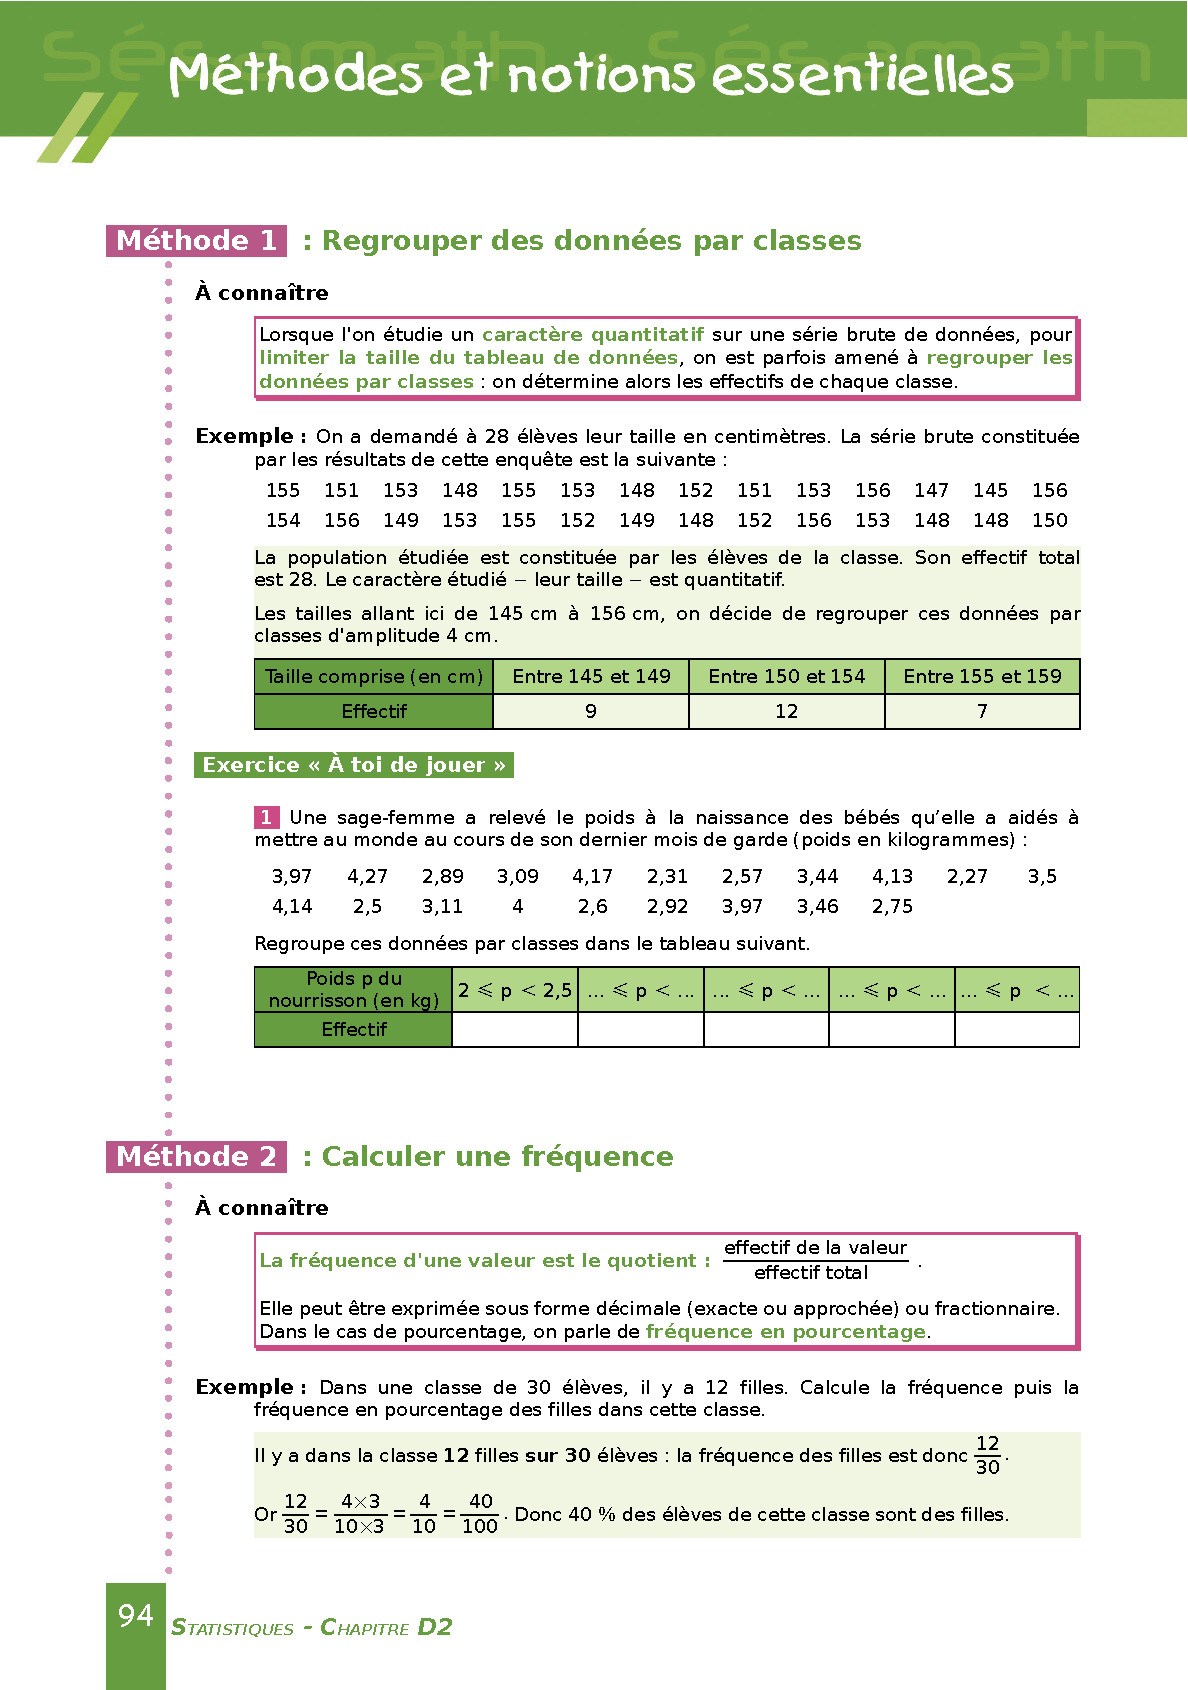
\includegraphics{sesamath5p94.pdf}
\end{center}
\begin{center}
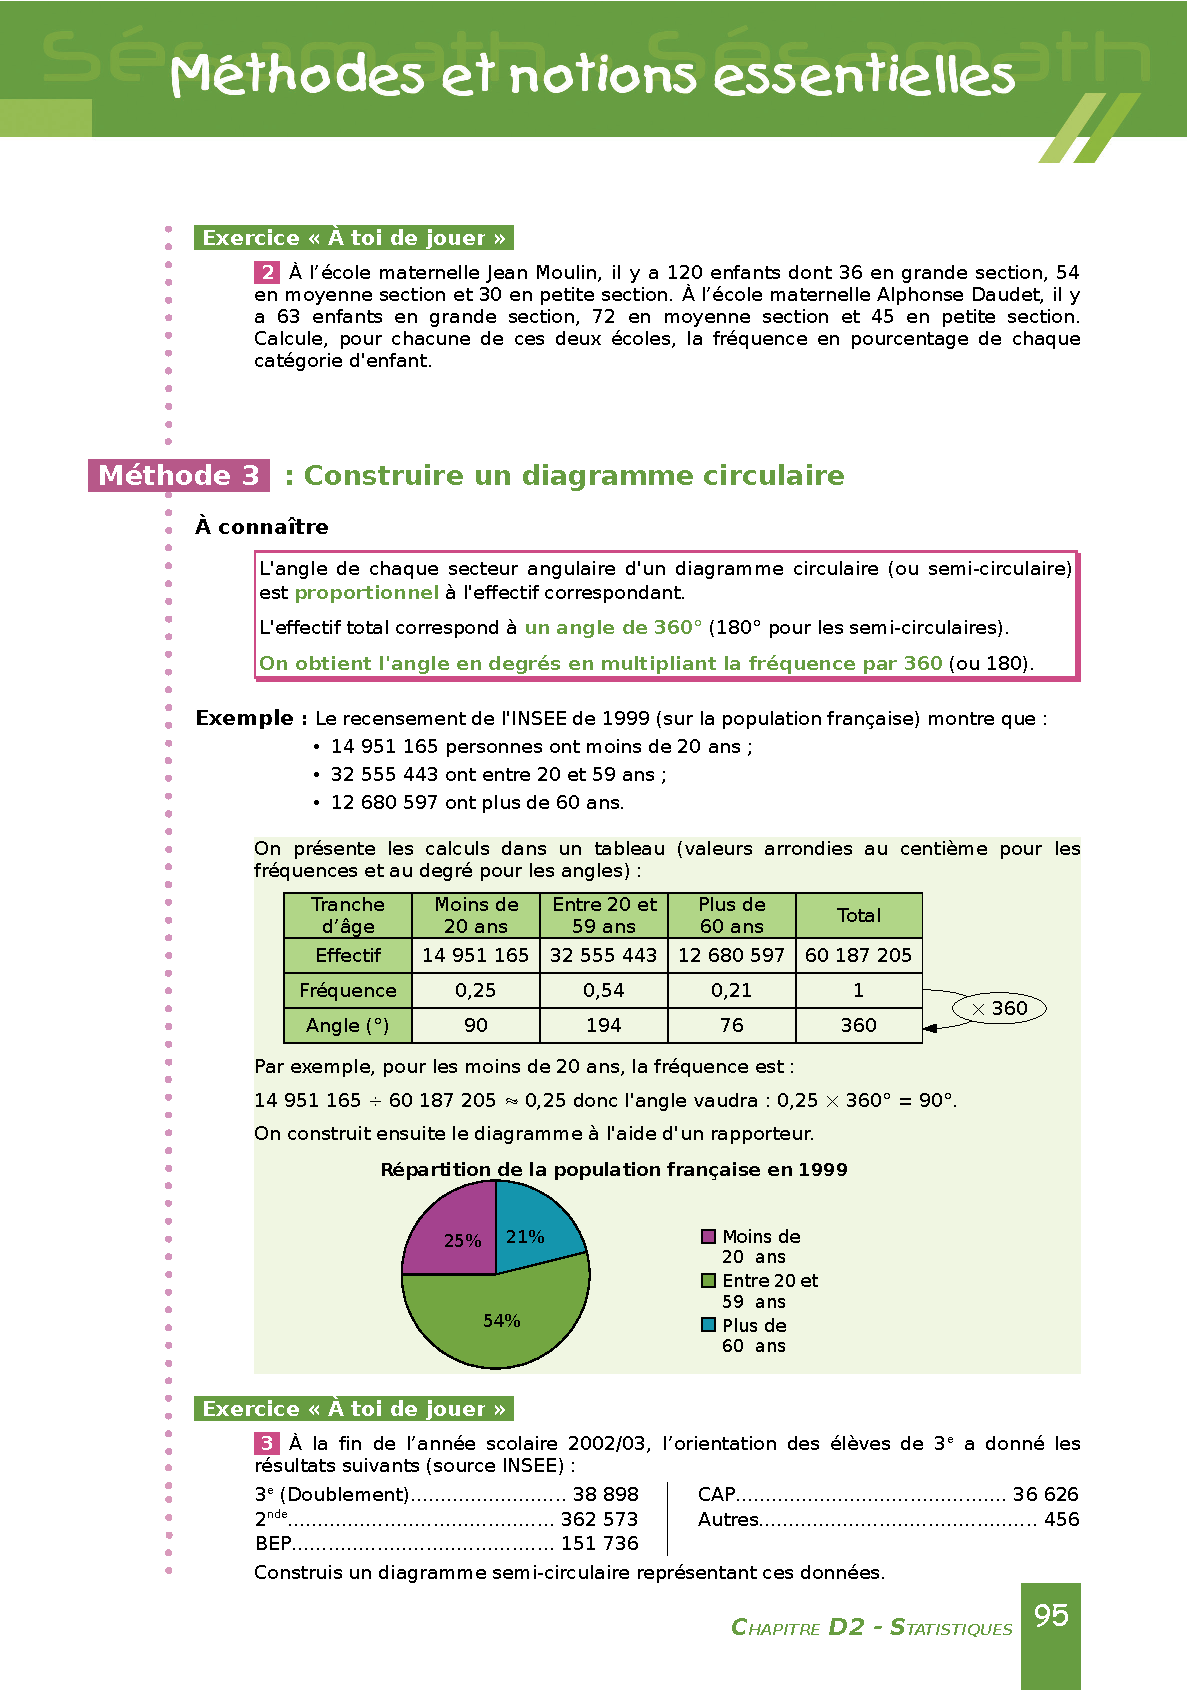
\includegraphics{sesamath5p95.pdf}
\end{center}


%+++++++++++++++++++++++++++++++++++++++++++++++++++++++++++++++++++++++++++++++++++++++++++++++++++++++++++++++++++++++++++ 
\section{Exemples : les devoirs}
%+++++++++++++++++++++++++++++++++++++++++++++++++++++++++++++++++++++++++++++++++++++++++++++++++++++++++++++++++++++++++++

Quelque statistiques sur les devoirs.

\vfill

Pour les 5A :

% les graphes viennent de phystricksTYIooYKqeNv.py

\begin{center}
   \input{Fig_CXWooOMPOQT.pstricks}
\end{center}

\vfill

Pour les 5B

\begin{center}
   \input{Fig_PJQooTWPTXV.pstricks}
\end{center}


Le couplage barème/compétences du DS numéro 6, 5A :

\begin{center}
   \input{Fig_TLEXooPDNwLRooONE.pstricks}
\end{center}

Le couplage barème/compétences du DS numéro 6, 5B :

\begin{center}
   \input{Fig_TLEXooPDNwLRooTWO.pstricks}
\end{center}
